\documentclass{beamer}
\usepackage{graphicx}
\usepackage{listings}

\usetheme{Madrid}
\usecolortheme{beaver}
\date[26 September 2025]{}

\title[We did it Patrick! We fixed traffic!]{Unconventional reinforcement learning on traffic lights with SUMO}
\subtitle{Master Degree in Computer Science}
% \author{Refolli~F.~865955}
\author[RF 865955]{Francesco~Refolli\\[10mm]{\small Supervisor: Prof. Giuseppe Vizzari}}
\logo{
\includegraphics[height=2.5cm]{logo_unimib.pdf}}

\newcommand{\putimage}[2] {
  \begin{figure}[H]
    \centering
    \includegraphics[width=#2\linewidth]{#1}
	\end{figure}
}

\newcommand{\putimagecouple}[4] {
  \begin{figure}[!htb]
    \centering
    \begin{minipage}{0.45\linewidth}
      \centering
      \includegraphics[width=\linewidth]{#1}
      \caption{#2}
    \end{minipage}
    \hspace{0.25cm}
    \begin{minipage}{0.45\linewidth}
      \centering
      \includegraphics[width=\linewidth]{#3}
      \caption{#4}
    \end{minipage}
  \end{figure}
}

% \begin{frame}
% \frametitle{Outline}
% \tableofcontents
% \end{frame}

\begin{document}

\frame{\titlepage}

\setbeamertemplate{logo}{}

\begin{frame}
  \begin{columns}
    \begin{column}{0.4\textwidth}
      \begin{figure}
        \centering
        
\includegraphics[width=1.0\textwidth]{figures/sumo-logo.png}
      \end{figure}
      \begin{itemize}
        \item Free and Open Source microscopic traffic simulator
        \item Developed at German Aerospace Center (DLR)
        \item Multimodal: cars, trams, bikes, pedestrians ...
        \item Highly customizable
      \end{itemize}
    \end{column}
    \begin{column}{0.6\textwidth}
      \begin{figure}
        \centering
        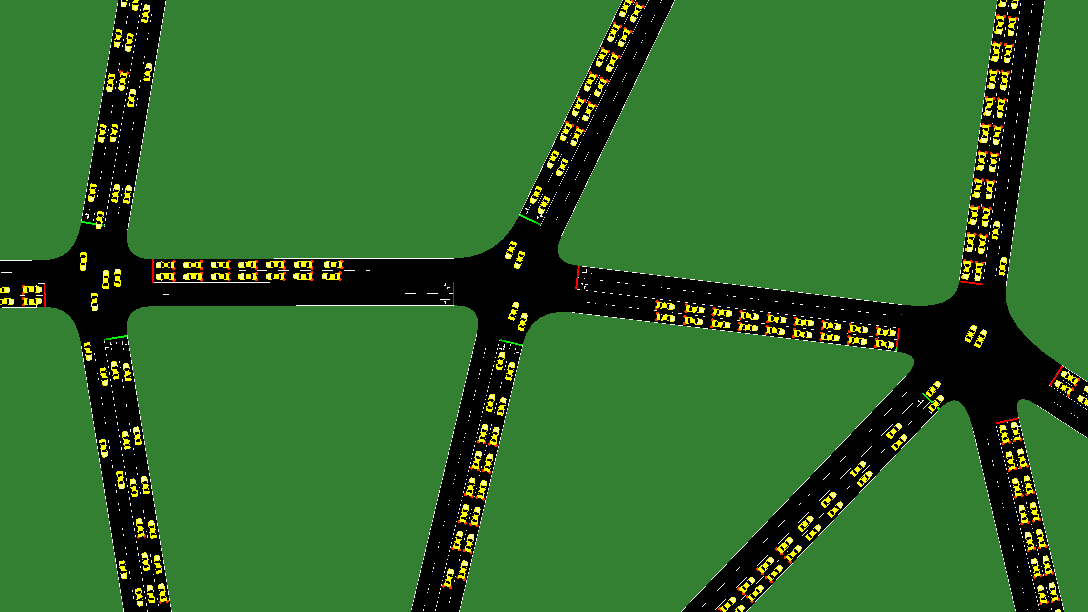
\includegraphics[width=1.0\textwidth]{figures/sumo-example.png}
      \end{figure}
      \begin{figure}
        \centering
        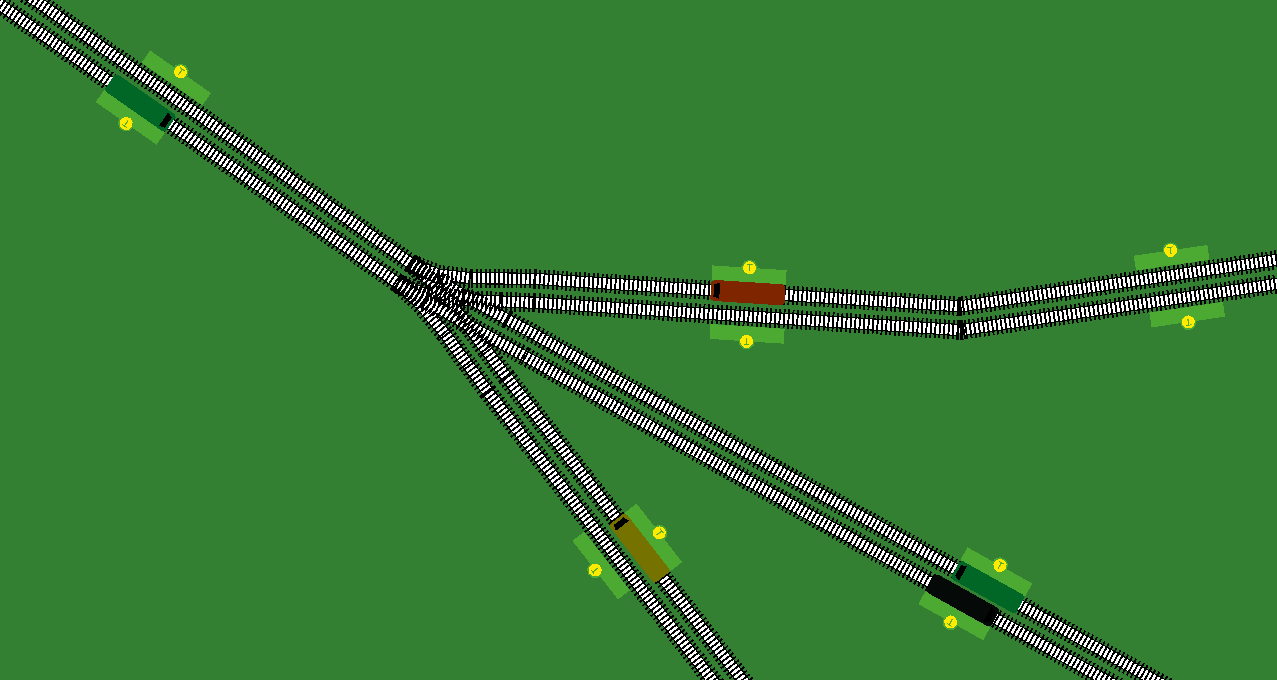
\includegraphics[width=1.0\textwidth]{figures/sumo-example2.png}
      \end{figure}
    \end{column}
  \end{columns}
\end{frame}

\begin{frame}
\frametitle{SUMO-RF: SUMO + Reinforcement Learning}
  A FOSS framework for Reinforcement Learning with SUMO developed as fork of \textit{LucasAlegre/sumo-rl} with a focus on modularity, flexibility and Multi Agent Learning.
  It also contains several utilities for format conversions, metrics analysis and plot, schematic-based demand generation and more.
  \begin{figure}
    \centering
    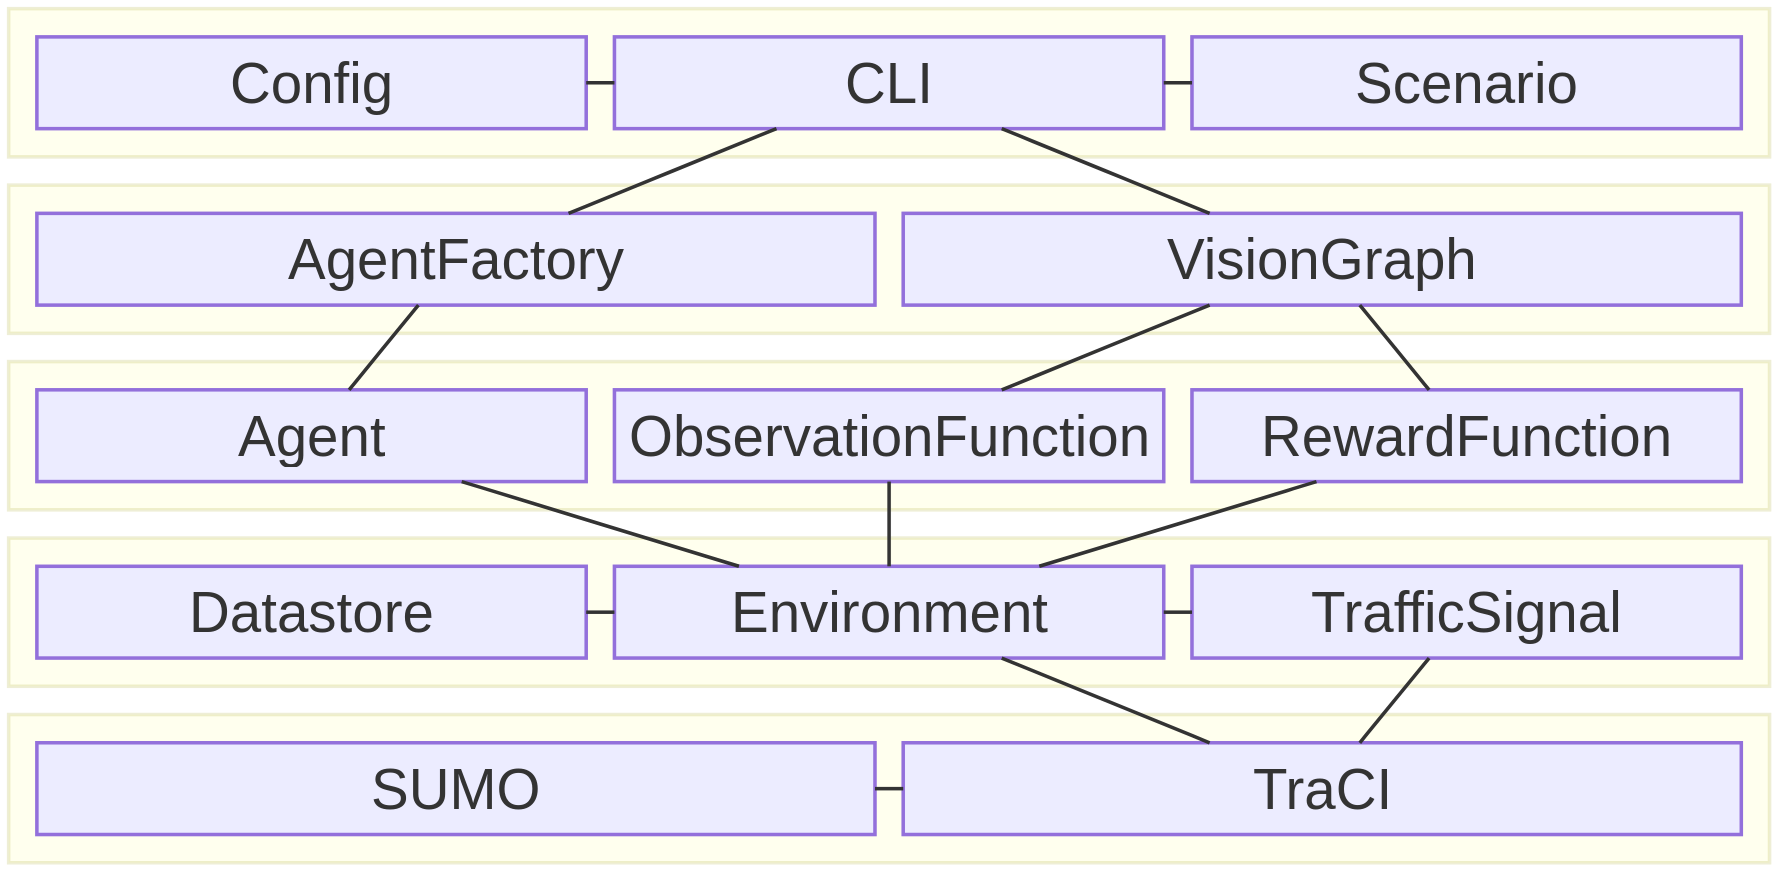
\includegraphics[width=0.8\textwidth]{figures/sumo-rf-architecture.png}
  \end{figure}
\end{frame}

\begin{frame}
\frametitle{The Agent Model}
  \begin{columns}
    \begin{column}{0.6\textwidth}
    {\small
    \begin{itemize}
      \item Each agent can control one intersection and at each step (every 5 seconds) it can choose the next phase of the intersection.
      \item Every action is automatically enforced by TrafficSignal with also an intermediate yellow phase.
      \item It receives an observation of the current condition and a reward proportional to the goodness of its behaviour.
      \item If the agent is "smart", it uses the collected data to improve itself!
    \end{itemize}}
    \end{column}
    \begin{column}{0.4\textwidth}
      \begin{figure}
        \centering
        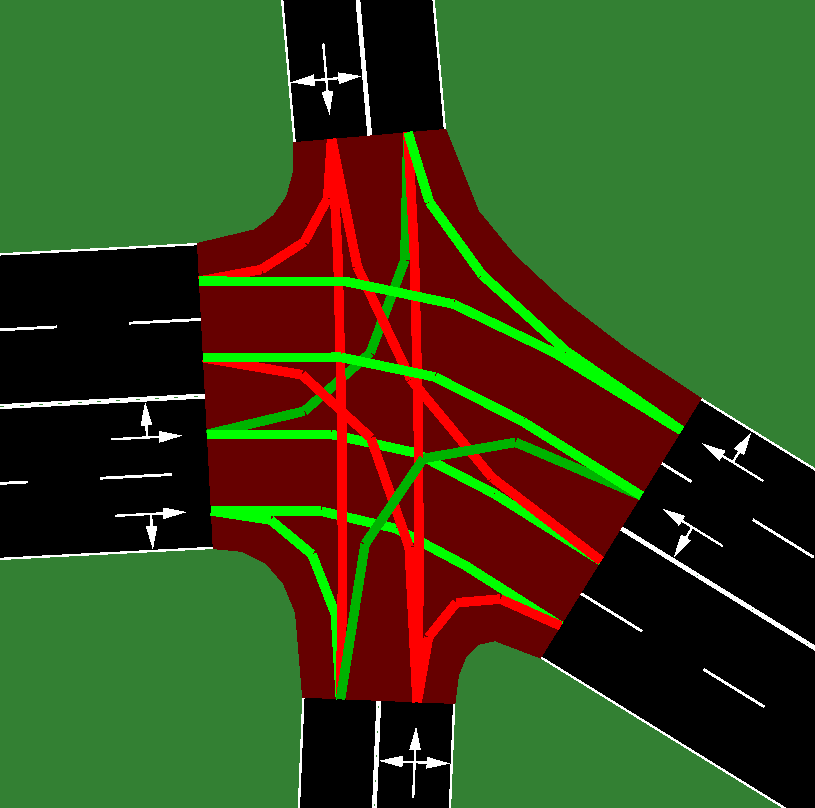
\includegraphics[width=1.0\textwidth]{figures/sumo-rf-agent.png}
      \end{figure}
    \end{column}
  \end{columns}
\end{frame}

\begin{frame}
\frametitle{The Global State}
  \begin{figure}
    \centering
    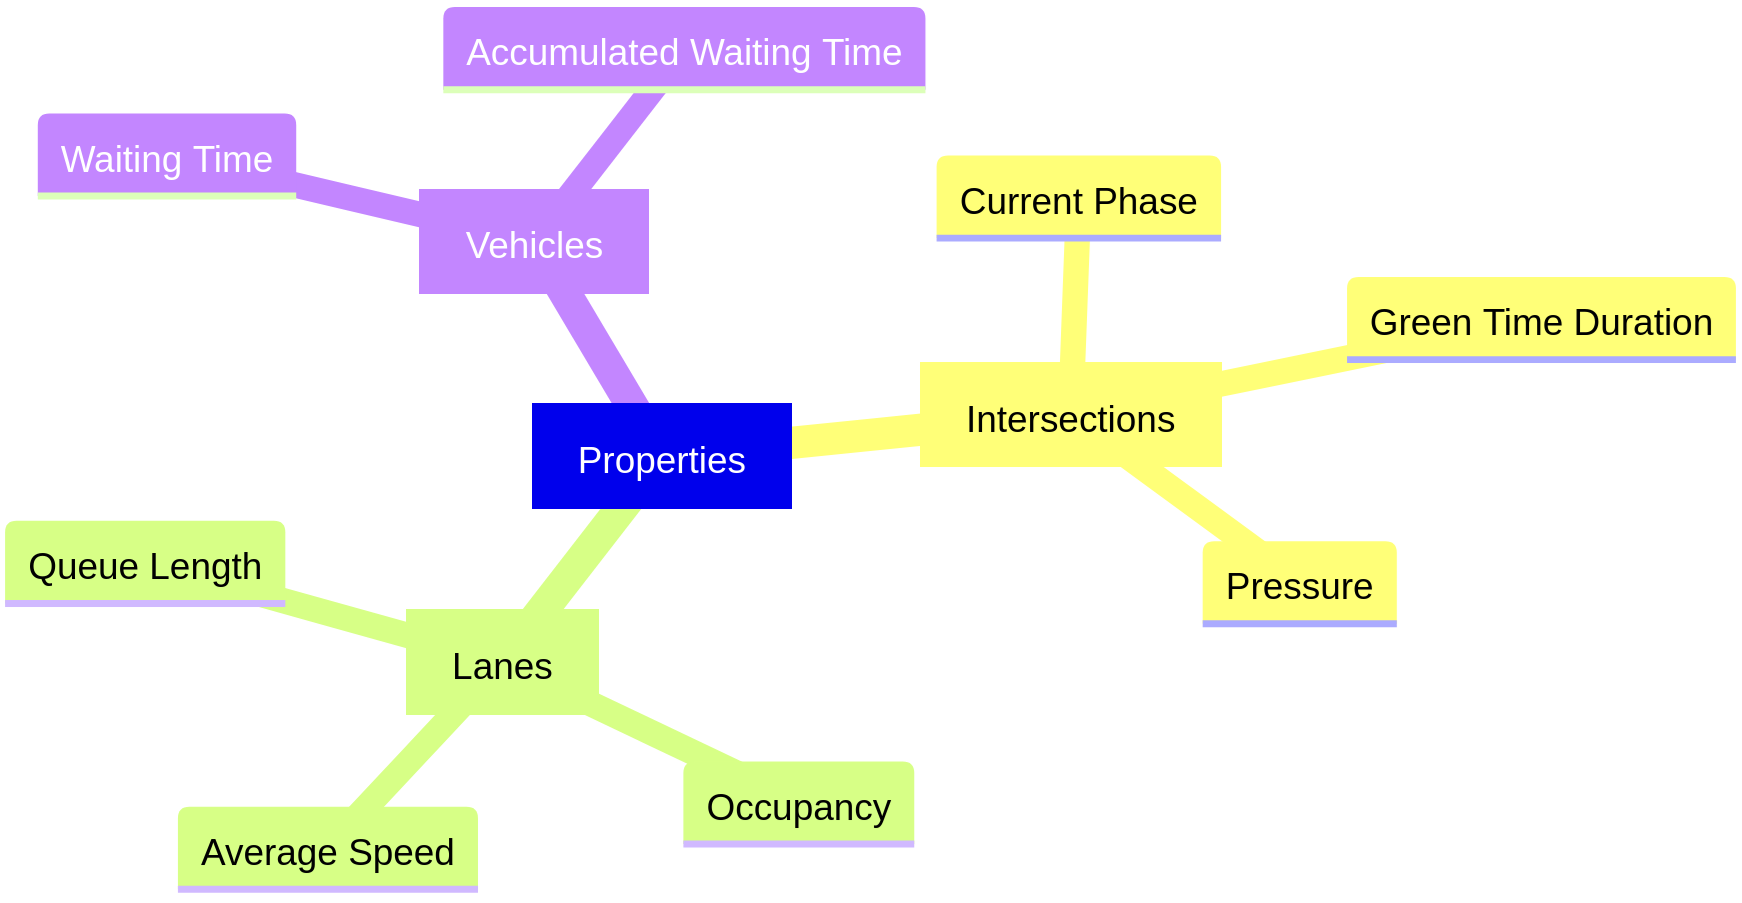
\includegraphics[width=1.0\textwidth]{figures/sumo-rf-properties.png}
  \end{figure}
\end{frame}

\begin{frame}
\frametitle{Observing and Rewarding}
  \begin{columns}
  \begin{column}{0.4\textwidth}
    \begin{figure}
      \centering
      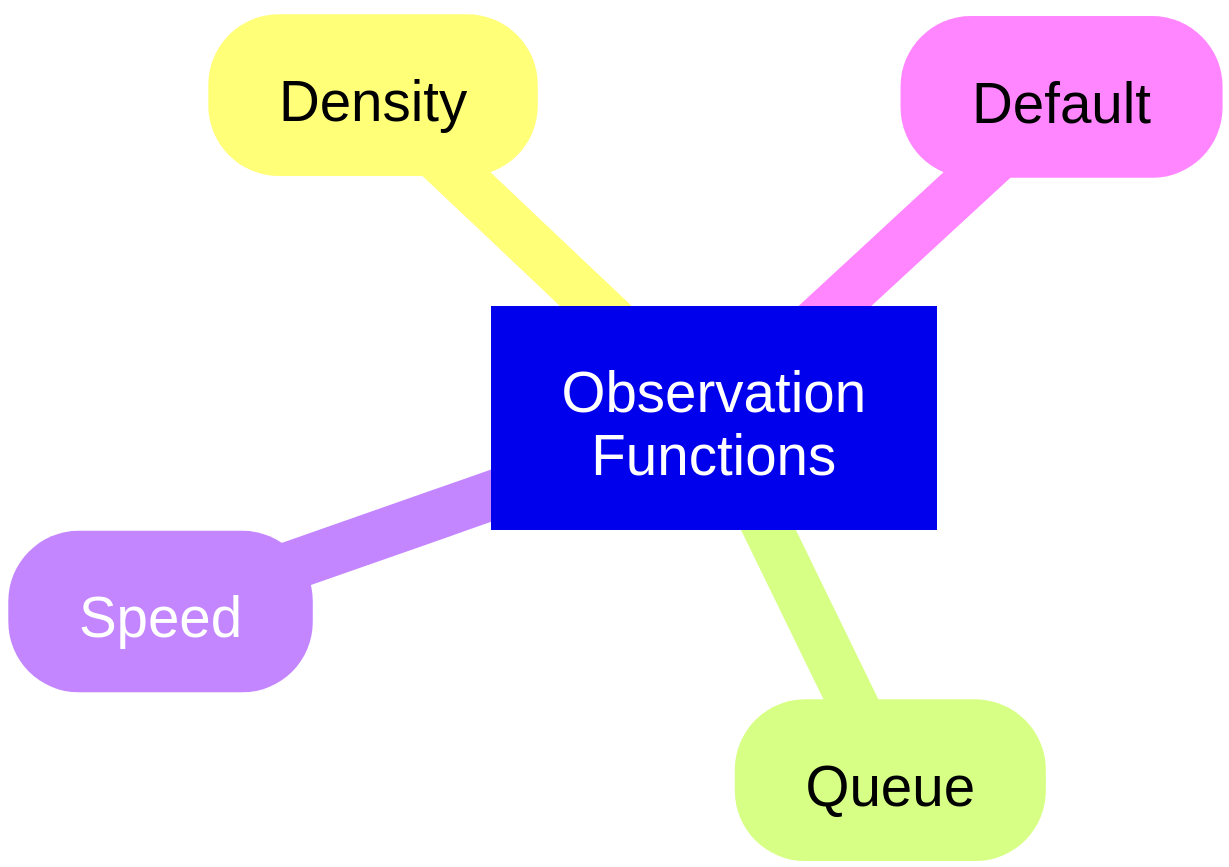
\includegraphics[width=1.0\textwidth]{figures/sumo-rf-observations.png}
    \end{figure}
  \end{column}
  \begin{column}{0.6\textwidth}
    \begin{figure}
      \centering
      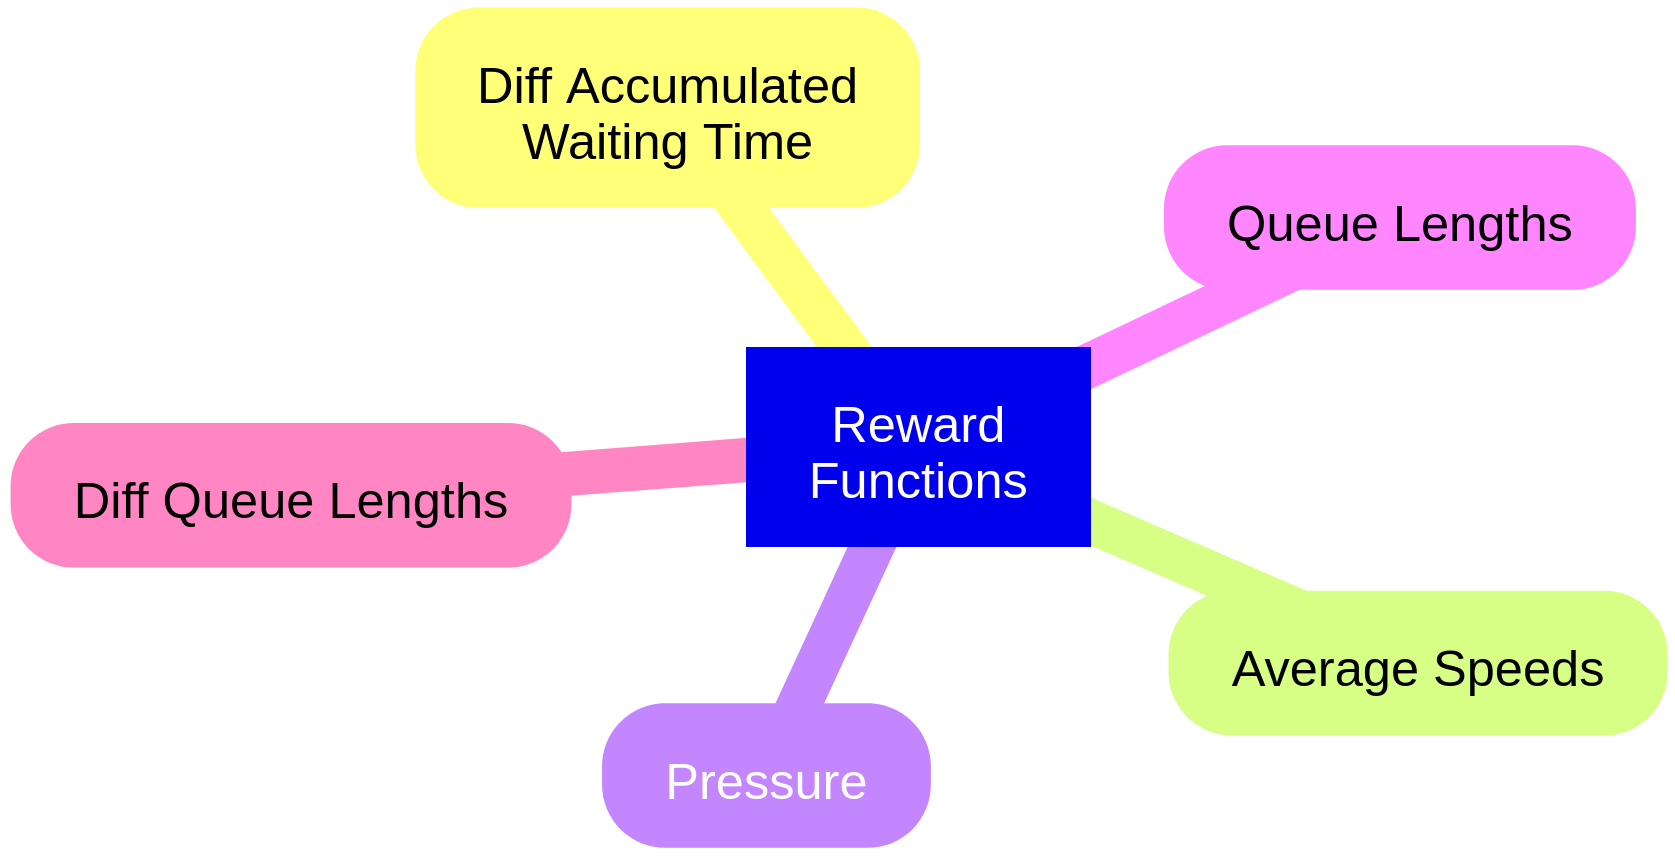
\includegraphics[width=1.0\textwidth]{figures/sumo-rf-rewards.png}
    \end{figure}
  \end{column}
\end{columns}
\end{frame}

\begin{frame}
\frametitle{Multi Agent Learning and "Shared-Views"}

  {\small
  No agent is isoled, they are all part of a whole and they influence each other with their own behaviour.
  What if an agent can \textit{sense} its surrounding area by sharing observations with neighbours? 
  What if an agent is \textit{rewarded} for its influence on surrounding area by sharing rewards with neighbours?}

  \begin{columns}
    \begin{column}{0.3\textwidth}
      \begin{figure}
        \centering
        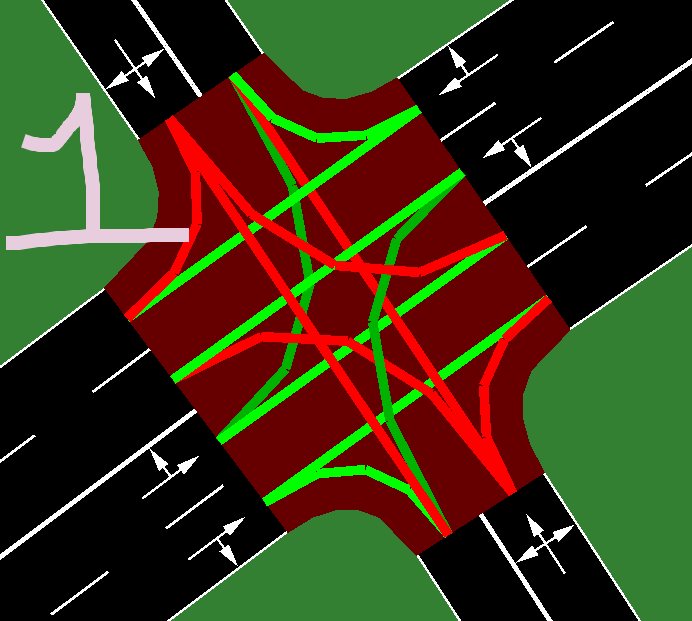
\includegraphics[width=0.75\textwidth]{figures/sumo-rf-tls-1.png}
      \end{figure}
    \end{column}
    \begin{column}{0.3\textwidth}
      \begin{figure}
        \centering
        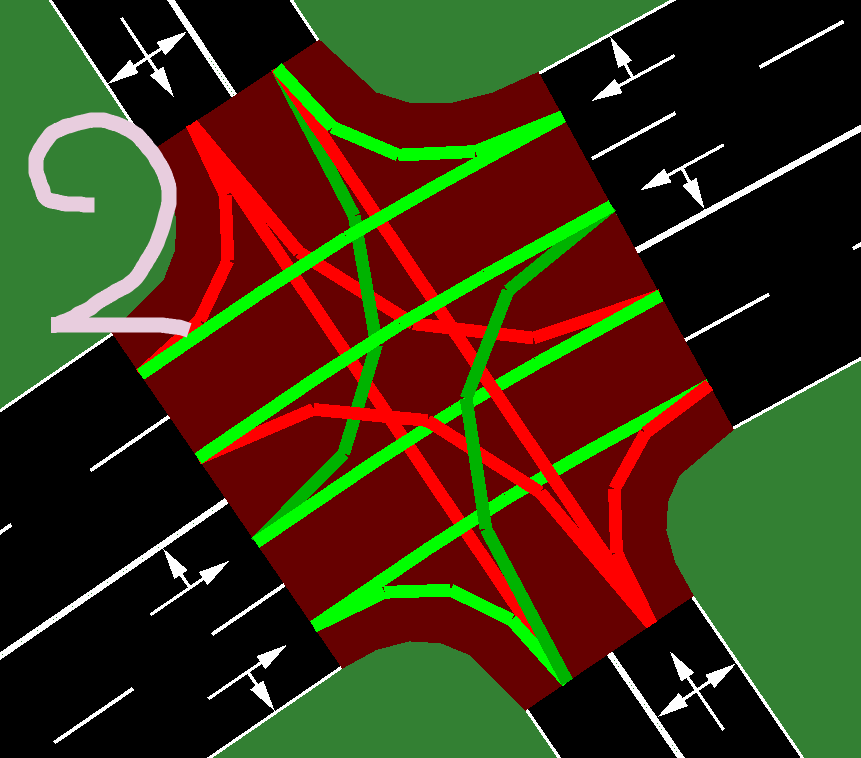
\includegraphics[width=0.75\textwidth]{figures/sumo-rf-tls-2.png}
      \end{figure}
    \end{column}
    \begin{column}{0.3\textwidth}
      \begin{figure}
        \centering
        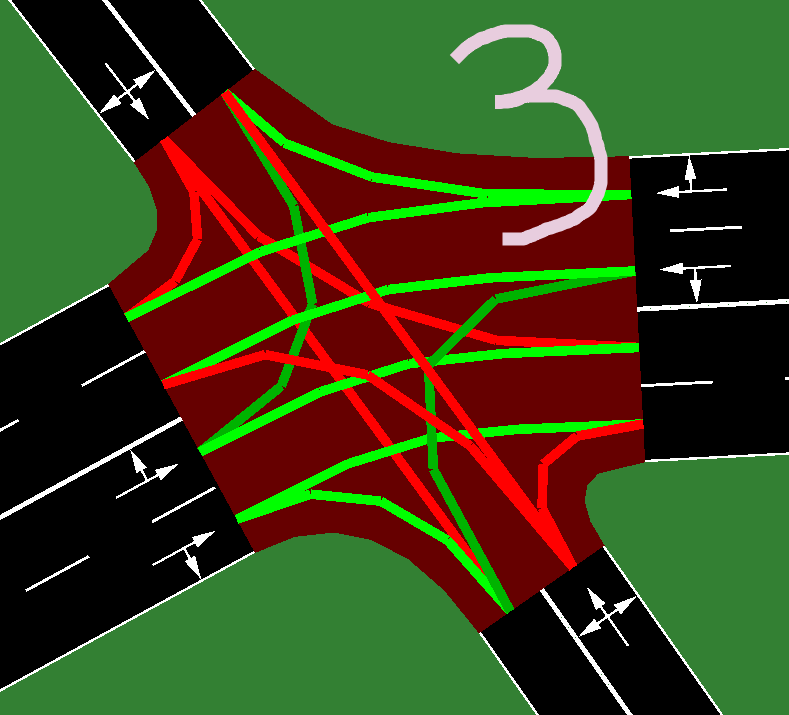
\includegraphics[width=0.75\textwidth]{figures/sumo-rf-tls-3.png}
      \end{figure}
    \end{column}
  \end{columns}
  \begin{columns}
    \begin{column}{0.5\textwidth}
      \begin{figure}
        \centering
        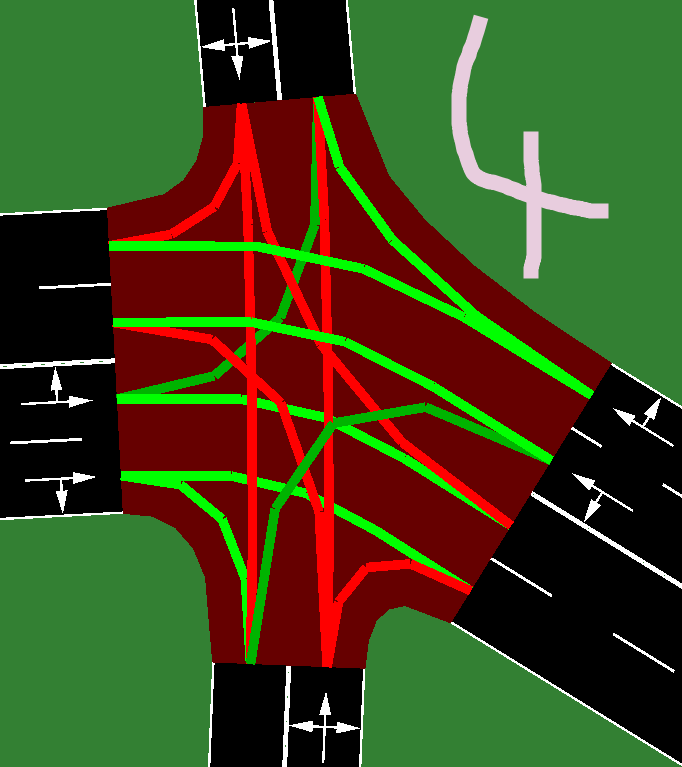
\includegraphics[width=0.35\textwidth]{figures/sumo-rf-tls-4.png}
      \end{figure}
    \end{column}
    \begin{column}{0.5\textwidth}
      \begin{figure}
        \centering
        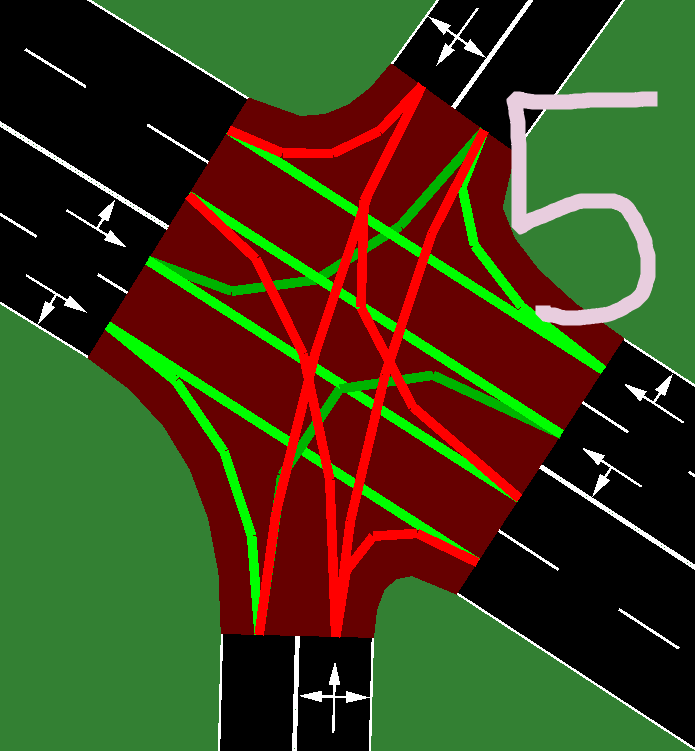
\includegraphics[width=0.35\textwidth]{figures/sumo-rf-tls-5.png}
      \end{figure}
    \end{column}
  \end{columns}
\end{frame}

\begin{frame}
\frametitle{Experience Engineering}
\end{frame}

%[fragile]
% \begin{small}
%   \begin{verbatim}
%   TOK = (£|\*|~|%(,[0-9.]+)?(,[0-9.]+)?|[A-Z][A-Z0-9]+)
%   EXP = ^([0-9]+,)?([0-9]+,)?TOK(,TOK)*$
%   \end{verbatim}
% \end{small}

\begin{frame}
\centering
\Huge
Thank You
\end{frame}

\end{document}
